\chapter{已有算法综述}
\label{cha:algrev}

关于距离几何问题的先驱性研究可以追溯到 Schoenberg 在 
1935年的研究~\cite{Schoenberg1935}, 
以及 Blumenthal ~\cite{Blumenthal1953} 和 Torgerson ~\cite{Torgerson1958} 的工作.
关于已有工作的一个简单的总结, 请参考 \cite{Fang2013} 中的表13.1. 
在本章中, 我们综述一些我们关注的算法, 主要是跟我们的研究方向的, 
但不企图覆盖所有算法.

例如, \cite{Qi2012} 就是一篇我们略过的有趣的文章, 它基于关于距离矩阵的
一个著名的结果 \cite{Schoenberg1935}, 研究秩约束的既约(变形后的)的距离矩阵.
对于有更深入兴趣的读者, 我们推荐参考 Liberti, Lavor, Maculan 和 Mucherino 2014年
发表在 SIAM Review 上的综述性文章 \cite{Maculan2014}, 文章比较全面而详实,
几位作者都对距离几何问题有着多年的研究和关注.

本章的结构如下.
在 \ref{sec:MatDcomp} 中, 我们介绍一个老的很特殊的矩阵分解算法,
它只能用来求解已知所有距离的距离几何问题, 但是之后很多算法的基础.
在 \ref{sec:Continuation} 中, 我们介绍全局光滑算法, 它对原误差函数进行光滑化处理,
期望抹去不重要的局部极小值点, 保留真正的全局极小值点.
在 \ref{sec:SDPalg} 中, 我们介绍多个基于半定规划的算法. 
半定规划在近年来得到广泛而深入的研究, 距离几何问题是其一个典型的应用例子.
应用半定规划, 我们能够比较方便地处理带不等式约束的问题.
\ref{sec:GB} 是我们介绍的重点, 我们在下一章提出的新的算法就是基于这些已有的算法,
所以我们会多费笔墨介绍算法的细节.
最后, 在 \ref{sec:otheralg} 中, 我们简要地提到其他一些比较重要的算法.


\section{矩阵分解算法 (Matrix Decompostion Method)}
\label{sec:MatDcomp}

Blumenthal 在 \cite{Blumenthal1953} 中提出了矩阵分解算法来求解
全部距离已知的距离几何问题. 全部距离是指点与点之间的两两距离都已知.
据我们所知, 这是针对这一问题最老的成熟的算法.
尽管它只能用来求解这一特殊情形, 但由于它是后续多个算法的关键步骤,
它仍然是非常重要的, 故而我们在此给出这一算法的细节.

由于整个结构\footnote{Structure, 在本文中指由点和边组成的二维或三维图形, 强调相对位置.}
在刚性变换(包括平移,旋转,和反射)\footnote{在本文中, 均指代平移, 旋转和反射变换中的一个或多个的复合, 后文将不特别说明.} 下保持不变,
不失一般性, 我们设 $x_n$ 在原点, 也就是 $x_n = (0,0,0)^T$. 
我们有 $d_{in} = \|x_i-x_n\| = \|x_i\|$. 
更进一步, 我们对等式 $\|x_i-x_j\| = d_{ij}$ 的两边同时取平方, 得到
\be \|x_i\|^2 - 2x_i^Tx_j + \|x_j\|^2 = d_{ij}^2, \quad i,j = 1,2,\ldots,n-1.\ee
将式中的 $\|x_i\|$ 用 $d_{in}$ 替代, 
并且把所有已知项移到同一边, 我们有
\be\label{eqn:sqrdist} x_i^Tx_j = (d_{in}^2 - d_{ij}^2 + d_{jn}^2 )/2, \quad i,j = 1,2,\ldots,n-1.  \ee
令 $X=(x_1,x_2,\ldots,x_{n-1})^T$ 为坐标矩阵,
其中$X^T$ 的每一列是一个点的坐标.
令 $B = (b_{ij}) = ((d_{in}^2 + d_{jn}^2 - d_{ij}^2)/2)$ 为距离矩阵的一个变换.
通过这些记号, (\ref{eqn:sqrdist}) 中的所有等式可以写成一个更紧凑的形式
\be XX^T = B. \ee
上面这个矩阵方程可以按如下的方式通过奇异值分解
(Singular Value Decomposition, 简称 SVD) 来求解.

\begin{Thm}{(Eckart, Young \cite{Eckart1936})}
令 $B=U\Sigma\Tran U$ 为奇异值分解, 
其中 $\Sigma$ 是所有奇异值按降序排列形成的对角矩阵. 
令 $V=U(:,1:k)$ 以及 $\Lambda=\Sigma(1:k,1:k)$, 
我们有 
\be X = V\Lambda^{1/2} \label{SVDsolution} \ee 
是下面这个问题的解
\be \min_{rank(X)\leq k} \|X\Tran X-B\|_F. \ee
\end{Thm}

在我们的应用中, 如果所有的距离都是精确的, 
并且不是所有原子都在同一个平面上, 那么矩阵 $B$ 将是秩 3 的, 
(\ref{SVDsolution}) 给出的就是精确解.
如果某些距离带有误差, 那么 $B$ 的秩通常大于 3, 
(\ref{SVDsolution}) 得到的就是最佳秩 3 逼近.

对于已知全部距离的距离几何问题, 
Dong 和 Wu \cite{Dong2002} 第一次给出了一个线性时间的算法.
顺便一提的是, 这也是几何构建系列方法的第一篇文章,
尽管名字 ``Geometric Buildup'' 是在之后的文章 \cite{Dong2003} 正式提出的.
关于这个方法的详细情况将在 \ref{sec:GB} 中给出.


\section{全局光滑算法 (Global Continuation Algorithm)}
\label{sec:Continuation}
如前所述, 误差函数通常都有大量的局部极小值点,
所以要直接找到原函数的全局极小值点是非常困难的.
在 \cite{More1997,More1999} 中, Mor\'e 和 Wu 提出了
一个全局光滑算法 \emph{dgsol} 来客服这个困难,
它的主要思想如下所述.

首先, 对原函数应用一个全局光滑化步骤. 
具体来说, 我们计算原误差函数与高斯密度函数的卷积.
直观地看, 这个过程把原函数在某一点的值用它周围点的均值所替代,
取均值的权重由高斯密度函数所决定, 以该点为中心成正太分布.
经过这一过程, 很多局部极小值点都被抹去了, 而真正的全局极小值点则被保留下来,
所以要找到光滑化之后的函数的全局解就容易得多了.
函数光滑化的程度是由一个参数 $\lambda$ 所控制的,
当 $\lambda$ 趋近于 0 的时候, 光滑化的函数逼近原函数.

算法的第二个关键技术叫做延续 (continuation), 
即逐步减小参数 $\lambda$ 到 0, 将上一步得到的解作为下一步的初始值,
应用局部优化算法如梯度法回溯求解, 最终找到原问题的解.
这里的思想跟求解非线性系统中的``同伦算法''非常接近,
都是将原问题化成结构类似但简单得多的问题, 再逐步回溯, 最终求解到原问题.

在 \cite{More1999} 中, 作者们给出了算法在一些小的蛋白质片段 (fragment)
上的计算结果, 表明 \emph{dgsol} 比重启动 (multi-start) 算法要有效和可靠得多.
值得一提的是, 重启动算法依靠某种方式 (如随机) 选择不同的初值点,
最后找一个最好的点作为解输出, 是求解全局优化的常用算法. 

全局光滑算法在理论上非常有意思, 但想用该算法来求解大规模的实际问题,
还需要进一步的深入研究.


\section{基于半定规划的算法 (SDP based algorithms)}
\label{sec:SDPalg}
半定规划 (Semidefinite Programming, 简称 SDP) 是近些年优化领域的一个研究热点.
关于它的理论已经非常成熟, 并且有很多易用的开源软件被开发出来,
如 SeDuMi 和 SDPT3 等\footnote{关于 SDP 的文献, 软件, 通知等资料参考
\url{https://www-user.tu-chemnitz.de/~helmberg/semidef.html}}. 
据我们所知, 关于距离几何问题的半定松弛算法 (SDP relaxation) 
最早是由 So 和 Ye 在 \cite{So2006} 中提出的, 
在这之后被众多学者进一步研究 \cite{Biswas2006-1,Biswas2008,Shamsi2010,Fang2013}. 
我们在下文简单总结关于这个算法的关键技术.

这些算法用到的一个基本模型是 (\ref{fun:abserr}). 
将 $|x|$ 用两个变量替代为 $x_+-x_- ~(x_+\geq 0,~x_-\geq 0)$, 
从而消去了函数中的非光滑项.
令 $X\in \Real^{n\times d}$ 是前文提到的坐标矩阵,
则 (\ref{fun:abserr}) 中的 $\|x_i-x_j\|^2$ 项可以重写为 $e_{ij}^TXX^Te_{ij}$, 
其中 $e_{ij}=e_i-e_j$. 
令 $Y=XX^T$ ,并松弛成 $Y\succeq XX^T$ \cite{Boyd1994}, 
这个线性矩阵不等式等价于
\be Z=\left(\ba{cc} Y & X \\ X^T & I \ea \right) \succeq \textbf{0}, ~~Z \textrm{ 是对称矩阵}.\ee
这样, (\ref{fun:abserr}) 的半定松弛可以写成一个以 $Z$ 为变量的
标准的半定规划问题. 注意, 我们要求 $Z$ 矩阵右下角 $d \times d$ 的子矩阵为单位阵.

半定松弛算法一个主要的优点是, 将此算法从求解等式约束的问题
推广到处理不等式约束不存在本质的困难, 
而对于其他算法来说, 这种推广并不容易, 甚至是不可能的.

这个方法的一个主要困难在于, 由于目前求解器 (solver) 的限制,
求解大规模 (超过几千个变量) 的半定规划问题的计算开销非常大.
考虑到这一点, Biswas, Toh 和 Ye 在 \cite{Biswas2008} 中第一次提出了针对
距离几何问题的分布式 (distributed) SDP 算法.
他们利用距离信息是局部及稀疏的特点, 基于距离矩阵,
将原图分割成了若干个带有重叠 (overlap) 区域的子图.
从而将大规模问题化解为了一些可以较快求解的小规模问题,
再将各子块拼接起来, 得到原图的结构. 
这种分布式策略在 \cite{Fang2013} 中也被用到, 
文章中他们进一步结合了从化学知识推断出的其他距离信息, 
并且设计了启发式 (heuristic) 策略来检测子块是否被精确定位,
这在分布式算法中是很关键的一点.
除了分布式以外, 另一种克服此困难的方法是将半定松弛进一步松弛 \cite{Wang2008} 
成基于结点或基于边的子问题, 它们都是可以高效求解的小规模问题.



\section{几何构建算法 (Geometric Buildup Method)}
\label{sec:GB}

几何构建算法是 Dong 和 Wu 在 \cite{Dong2002} 中首次提出来的, 
针对的是已知全部距离的情形, 
随后被推广到处理稀疏数据 \cite{Wu2006}. 
该算法在 \cite{Wu2008,Sit2009} 中被进一步完善, 
线性和非线性最小二乘近似 (linear and nonlinear least square approximation)
被提出来防止误差的累积.

几何构建算法基于这样一个事实: 在 $d$ 维空间中,
一个点通常可以被 $d+1$ 个到该点的距离唯一确定.
例如, 在三维空间中, 两个到固定点的距离可以确定\footnote{意指未知点到固定点的距离要满足所给距离, 这样的点形成的集合.}
一个圆 (假设两圆相交但不相切); 
而三个距离一般可以确定两个点, 四个距离则可以唯一确定一个点.
当然, 我们要求原来的四个固定点不在同一个平面上.
一般地, 我们要求 $d+1$ 个固定点不在同一个超平面上.
基于这些观察, 我们很自然地就可以得到集合构建算法的核心思想:
先确定四个点, 在逐步一个一个地确定剩下的点.
为了文章的完整性, 以及为了便于讨论并在下一章给出我们的新算法,
我们在此给出该算法的详细步骤.

\subsection{确定最初的四个点}
我们暂时考虑已知的是精确距离的情形.
首先找到形成团 (clique) 的四个点, 团的意思是这些点所构成的子图是一个完全图,
也就是这些点之间的两两距离都已知.
注意到在平移, 旋转和反射变换下, 所有的距离都保持不变,
不失一般性, 我们把第一个点设为原点---$(0,0,0)^T$, 
第二个点位于 x 的正半轴\footnote{为了方便起见, 我们称三个坐标轴为 x, y z 轴.},
其坐标为 $(d_{12},0,0)^T$,
第三个点位于 xy 平面的第一象限,
再随意选定第四个点位于两种可能性中的一个. 
我们略过这些简单的几何计算细节, 它们也可以在 \cite{Dong2002} 中找到.

\subsection{构建 (Buildup) 步: 确定一个未知点}
如前所述已经确定的四个点叫做基准点, 
我们再依次确定剩下的点, 正如从几块基石上一砖一瓦地盖起高楼大厦.

我们在此给出一个构建步的细节. 
我们把坐标已经确定的点叫做已知点, 剩下的点叫做未知点.
前文已经提到, 我们需要至少四个到已知点的距离来确定一个未知点.
假定点 $j$ 是要被定位的点, 它到四个已知点 $x_i ~(i=1,2,3,4)$ 的距离已知, 
也就是说, 我们有
\be \|x_i-x_j\| = d_{ij}, \quad i = 1,2,3,4.\ee
对这些等式的两边取平方, 得到
\be \|x_i\|^2 - 2x_i^Tx_j + \|x_j\|^2 = d_{ij}^2, \quad i = 1,2,3,4. \ee
注意, 在这些方程中, $x_j$ 是变量, 而 $x_i$ 是已知的.
现在我们有四个方程, 我们依次用后一个方程减去前一个方程\footnote{这不是唯一的方式, \cite{Dong2003} 讨论了不同的减去方式, 
以及在实际计算中可能不同的数值稳定性. 
我们可以在这多种方式中选择最优的一种, 但计算量也会成培增加.},
得到
\be 2(x_{i+1}-x_i)^Tx_j =(\|x_{i+1}\|^2-\|x_i\|^2) - (d_{i+1,j}^2-d_{ij}^2),\quad i = 1,2,3. \label{eqn:Ab} \ee
令 $A$ 为一个矩阵, $b$ 为一个列向量, 其中
\be A = 2\left[\ba{c} (x_2-x_1)^T \\(x_3-x_2)^T\\(x_4-x_3)^T \ea \right],
~b=\left[\ba{c}(\|x_2\|^2-\|x_1\|^2)-(d_{2j}^2-d_{1j}^2)\\
(\|x_3\|^2-\|x_2\|^2)-(d_{3j}^2-d_{2j}^2)\\(\|x_4\|^2-\|x_3\|^2)-(d_{4j}^2-d_{3j}^2)\ea \right],\label{eqn:dataAb}\ee
则 (\ref{eqn:Ab}) 中的等式可以写成一种更紧凑的形式
\be Ax_j=b. \label{eqn:Axb} \ee
如果这些已知点不都在同一个平面上, 那么 $A$ 是非奇异的,
未知点可以被唯一确定, 其精确解为 $x_j=A^{-1}b$.

\subsection{线性最小二乘}\label{LLS}
如果给定的距离是带误差的, 那么仅仅利用四个距离, 
求解方程 $Ax_j=b$ 并不能给出一个精确的解.
事实上, 从错误的距离信息出发, 我们几乎永远不可能得到``正确的''解,
但我们还是希望得到一个尽可能准确的解.
一种自然的处理办法就是, 利用尽可能多的距离, 从而得到一个合理的解.

假设我们已知的是 $l ~(l\geq 4)$ 个距离, 
那么我们就可以不求解等式方程 (\ref{eqn:Axb}), 
而是求解一个线性最小二乘问题
\be \min_{x_j} \|Ax_j-b\|, \ee
其中, $A$ 和 $b$ 是按照 (\ref{eqn:dataAb}) 类似的方式构成的, 
但都有 $l-1$ 行. 
这就是 Wu, Wu 和 Yuan 在 \cite{Wu2008} 中提出的
带线性最小二乘的几何构建方法, 更具体的细节可以参看原文.
我们在本文中将此方法简记为 GB-LLS.

\subsection{非线性最小二乘}\label{NLS}
注意到, 在 GB-LLS 中, 只有未知点到已知点之间的距离
(图 \ref{fig:DistEx} 中的粗实线) 被用到,
但是我们通常还会知道一些已知点之间的距离 (图 \ref{fig:DistEx} 中的实线). 
为了用到这部分信息, 在 \cite{Wu2008} 中, 
作者们进一步提出了带非线性最小二乘\footnote{这里并不算严格意义的``最小二乘''问题, 此处是类比于前一个算法的叫法.}
的几何构建算法, 我们在本文中记为 GB-NLS.

\begin{figure}[htb!]
  \centering
  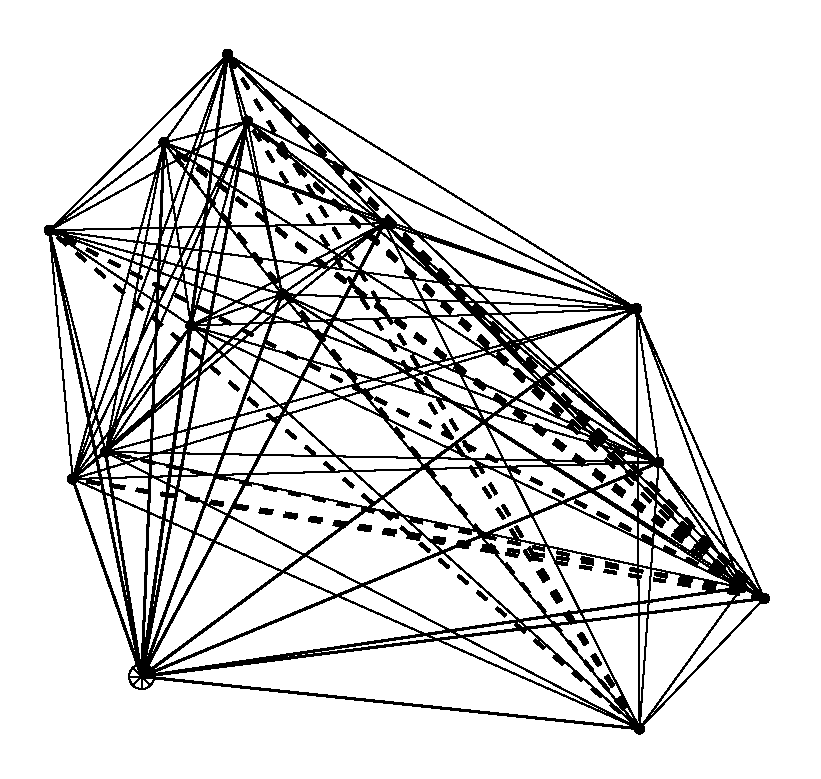
\includegraphics[width=0.4\textwidth]{DistEx.eps}\\
  \caption{GB-NLS 中的一步所涉及到的子图. 星型点: 未知点, 实心点:已知点.
  实线和粗实线: 已知的距离, 虚线: 计算的距离.}\label{fig:DistEx}
\end{figure}

在 GB-NLS 中, 首先是通过已知点的坐标计算
已知点之间未被测量的距离 (图 \ref{fig:DistEx} 中的虚线).
由此, 这 $l+1$ 个点所形成的子图, 其所有的两两距离都已知, 
从而可以利用 \ref{sec:MatDcomp} 中所介绍的矩阵分解算法来求解子问题.
求解之后需要通过旋转平移将这 $l+1$ 个点在子坐标系中的坐标变换到
原全局坐标系, 细节将在后文 (??) 给出.
这一步可以确定未知点 $j$, 与此同时对已经确定的 $l$ 个点进行微调. 
通常这个调节是细微的, 但是对整个算法却是非常重要的,
因为它提供了一个根据新利用到的距离改进原本不精确的定位的机会,
而不像在 GB-LLS 中, 一个点一旦被确定, 就永远地固定了.


\section{一些其他算法}
\label{sec:otheralg}





